\section{Testing plan}

The main goals of this performance testing plan are:
\begin{itemize}
  \item to find out whether the usage of LSM implies some sort of performance penalty;
  \item to identify possible improvements when embedding WebAssembly in another language.
\end{itemize}

\noindent
For a given program written in Rust, the following configurations are tested:
\begin{itemize}
  \item a native binary, compiled by \texttt{rustc} and run as an executable under the following conditions:
        \begin{itemize}
          \item without a sandbox;
          \item sandboxed with Landlock (in this case, the program has to be modified - an example is visible in Listing \ref{lst:test-program-landlock-example});
          \item sandboxed with eBPF.
        \end{itemize}
  \item a WebAssembly binary obtained by the same Rust program and run:
        \begin{itemize}
          \item directly by the \textit{Wasmtime} command line tool;
          \item by the WASM runtime developed in Section \ref{sec:restricting-wasi-landlock} and restricted with Landlock;
          \item by the WASM runtime developed in Section \ref{sec:restricting-wasi-landlock} and restricted with
                eBPF\footnote{In this case, Landlock is disabled.}.
        \end{itemize}
\end{itemize}

The first three cases, where the native binary is tested, will be analysed in Section \ref{sec:landlock-vs-ebpf-native}
in order to find eventual differences between the sandboxes given by Landlock and eBPF.
The latter three cases will be analysed in Section \ref{sec:landlock-vs-ebpf-wasm} to see
how the sandboxed WASM runtime compares to \textit{Wasmtime}.

\vspace*{0.5cm}
\begin{code}[language=Rust, caption=An example of a program restricted with Landlock., label=lst:test-program-landlock-example]
use anyhow::Result;
use landlock::*;

const ACCESS: BitFlags<AccessFs> =
  make_bitflags!(AccessFs::{ ReadFile });

fn main() -> Result<()> {
    let path_fd = PathFd::new("input-file.txt")?;
    
    let path_beneath = PathBeneath::new(path_fd)
      .allow_access(ACCESS);
    let _ = Ruleset::new()
        .handle_access(AccessFs::from_all(ABI::V1))?
        .create()?
        .add_rule(path_beneath)?
        .restrict_self()?;

    // Here goes the main code
    // ...

    Ok(())
}
\end{code}

\clearpage
\subsection{System and hardware}

The system and hardware used for both the development of the project described in Section \ref{sec:restricting-wasi-landlock}
and the performed test is as follows:
\begin{itemize}
  \item Arch Linux \cite{arch-linux} as the operating system, more specifically the 2022.05.01 version;
  \item an Intel Core i5-7200U quad-core with a clock rate of 2.5 GHz;
  \item 8 GB of RAM;
  \item a 120 GB solid state disk.
\end{itemize}

The choice of the operating system is mainly dictated by the fact that Arch Linux has both Landlock and eBPF active
out of the box, removing the need to compile the Linux kernel with the necessary flags to enable these
functionalities.

\subsection{Tests' description}
\label{sec:performance-test-description}

The performed tests are:
\begin{itemize}
  \item a purely computational program, given by the sorting of 10000 random numbers as in Listing \ref{lst:sorting-test-rust},
        in order to measure only the computational impact of the various methods;
  \item a simple reading of files of various sizes as in Listing \ref{lst:reading-test-rust}, with only the necessary permissions enabled on
        a case-by-case bases, in order to test the sandbox provided and how they fare against native binaries.
\end{itemize}

The reading file test is repeated with different file sizes\footnote{Randomly generated by using \texttt{/dev/urandom}.},
which are $100$ KB, $1$ MB, $10$ MB and $100$ MB. By doing this, it is possible to see how performance
varies when dealing with progressively large files. Moreover, an additional empty file is used to
test the overhead on the pure opening of a file.

\vspace*{0.5cm}
\begin{code}[language=Rust, caption=The tested ``sorting program''., label=lst:sorting-test-rust]
use rand::Rng;

fn main() {
  let mut rng = rand::thread_rng();
  let mut vec: Vec<i32> = Vec::new();

  for _ in 0..10000 {
    vec.push(rng.get::<i32>());
  }

  vec.sort();
}
\end{code}

\begin{code}[language=Rust, caption=The tested ``reading program''., label=lst:reading-test-rust]
fn main() {
  let content = std::fs::read("input-file.txt");
  match content {
      Ok(c) => println!("{}", c.len()),
      Err(_e) => std::process::exit(1),
  }
}
\end{code}

\subsection{Performance indicators}

The main performance indicators will be the mean execution time, measured in milliseconds, together with its
standard deviation in order to compensate for variability.
These measures are always obtained from a sample of 100 runs, executed and measured by \texttt{hyperfine},
a command-line benchmarking tools \cite{hyperfine}, and finally saved to a
JSON file.

In this chapter, we define for brevity $\mu_x$ to be the mean of the method $x$ and $\sigma_x$ to be
the standard deviation of the method $x$.

\section{Comparison between different sandboxes}

In this section we will look at what impact different LSMs bring on a program,
be it a native binary or a WebAssembly binary run through some kind of runtime.

In Table \ref{table:lsm-impact-native} are present all execution times for a native binary,
compiled directly with \texttt{rustc} and run both unrestricted (\textit{Native}) and restricted
with different LSMs (\textit{Landlock} and \textit{eBPF}).

On the other hand, Table \ref{table:lsm-impact-wasm} is about running a WebAssembly binary through
\textit{Wasmtime} without any restriction, or through the WASM runtime developed in Section \ref{sec:restricting-wasi-landlock}
and restricted with Landlock (\textit{WL}) or eBPF (\textit{WeBPF}).

\begin{table}
  \centering
  \csvreader[
    tabular={|l|r|r|r|r|r|r|},
    table head = \hline
      \textit{Test type}
      & $\mu_\mathrm{Native}$   & $\sigma_\mathrm{Native}$
      & $\mu_\mathrm{Landlock}$ & $\sigma_\mathrm{Landlock}$
      & $\mu_\mathrm{eBPF}$     & $\sigma_\mathrm{eBPF}$ \\ \hline\hline,
    late after line = \\ \hline,
    head to column names,
  ]{test-data/native-landlock-ebpf.csv}{}
  {\type & \mnative & \snative & \mlandlock & \slandlock & \mebpf & \sebpf}
  \caption{Execution times of a native binary under different restrictions (in ms).}
  \label{table:lsm-impact-native}
\end{table}

\begin{table}
  \centering
  \csvreader[
    tabular={|l|r|r|r|r|r|r|},
    table head = \hline
      \textit{Test type}
      & $\mu_\mathrm{Wasmtime}$   & $\sigma_\mathrm{Wasmtime}$
      & $\mu_\mathrm{WL}$ & $\sigma_\mathrm{WL}$
      & $\mu_\mathrm{WeBPF}$     & $\sigma_\mathrm{WeBPF}$ \\ \hline\hline,
    late after line = \\ \hline,
    head to column names,
  ]{test-data/wasm-landlock-ebpf.csv}{}
  {\type & \mnative & \snative & \mlandlock & \slandlock & \mebpf & \sebpf}
  \caption{Execution times of a WASM binary under different restrictions (in ms).}
  \label{table:lsm-impact-wasm}
\end{table}

\subsection{A computational-heavy program}

Let's take a look at how restricting a purely computational-heavy program, namely the sorting of 
10000 random numbers showin in Listing \ref{lst:sorting-test-rust}, affects its performance.
Comparing the first lines of Table \ref{table:lsm-impact-native} and Table \ref{table:lsm-impact-wasm},
it is immediately apparent that using a LSM to restrict a binary, be it native or WebAssembly, worsen performance.

When dealing with a native binary, \textit{Landlock} has a lower overhead than \textit{eBPF} (an average
of $1.03$ ms for Landlock against an average of $2.30$ for eBPF), as is visible in Figure \ref{fig:distribution-sorting-native}.
This could be due to how the two sandoxes are enforced:
\begin{itemize}
  \item Landlock is directly available as a C library in the Linux kernel, so the communication between
        the program and the relative LSM can be as simple as multiple function calls;
  \item on the other hand, eBPF needs to have an active server\footnote{As highlighted in Section \ref{sec:restricting-wasi-ebpf}.},
        so the communication has to undergo a message exchange between processes.
\end{itemize}
By following this line of reasoning, it is expected that Landlock should be a little faster than eBPF.
Moreover, eBPF is more complex than Landlock since it allows more control on what
can and cannot be done by a running program, hence it has to deal with a higher complexity.
The overhead of eBPF, however, becomes smaller and smaller when measured in percentage as the execution times get higher.
This means that for small and fast programs the slow-down could become apparent if they get called many times
in a short period of time, while for slower program called with less frequency this should be negligible.

When dealing with a WebAssembly binary, the computational-heavy program is noticeably slower
compared to the native binary execution times, either unrestricted or restricted, as shown in Figure \ref{fig:distribution-sorting-wasm}.
The same reasoning applied before is valid here too - eBPF is a little slower than Landlock, with a overhead
of about $1$ ms.
However, restricting a WASM binary with the runtime developed in Section \ref{sec:restricting-wasi-landlock}
introduces a constant overhead of around $30$ ms with respect to \textit{Wasmtime}.
Since it is visible in Table \ref{table:lsm-impact-native} that Landlock is quite close to
unrestricted performance on average, and because Landlock was disabled when running
the tests combining WASM and eBPF, this extra time could be due to how the WASM module gets
interpreted by the library provided by \textit{Wasmtime}.

\begin{figure}[ht]
  \centering
  \begin{subfigure}[b]{0.32\textwidth}
    \centering
    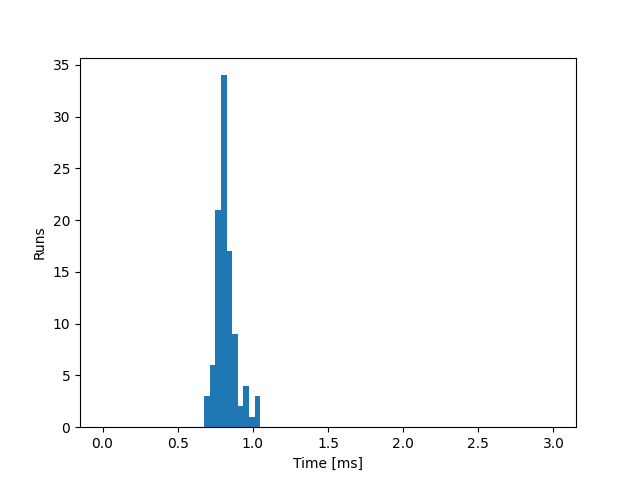
\includegraphics[width=\textwidth]{tests/sorting.native.png}
    \caption{Native}
  \end{subfigure}
  \begin{subfigure}[b]{0.32\textwidth}
    \centering
    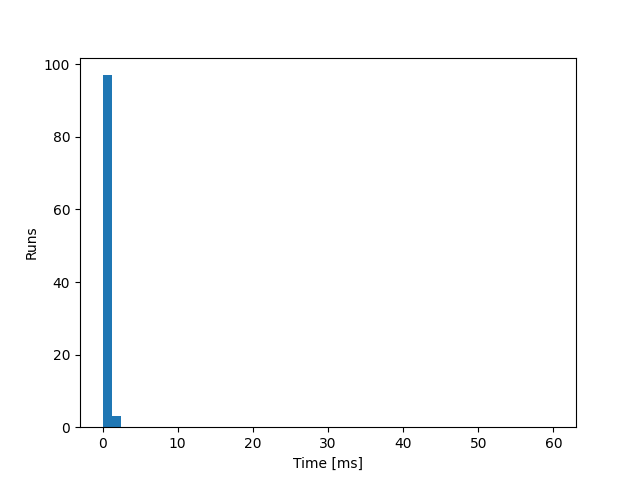
\includegraphics[width=\textwidth]{tests/sorting.native-landlock.png}
    \caption{Landlock}
  \end{subfigure}
  \begin{subfigure}[b]{0.32\textwidth}
    \centering
    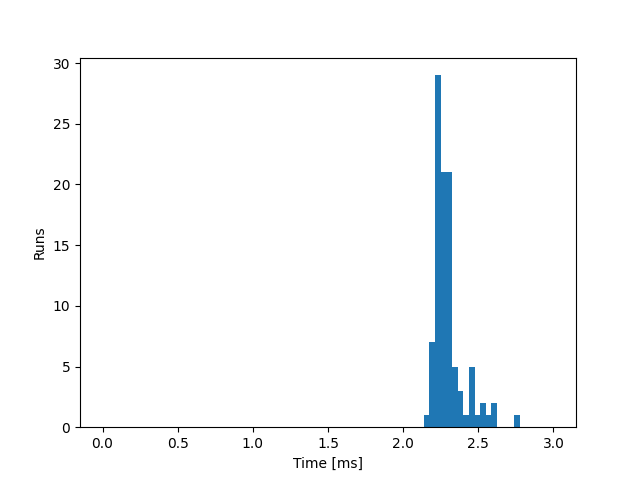
\includegraphics[width=\textwidth]{tests/sorting.native-bpf.png}
    \caption{eBPF}
  \end{subfigure}
  \caption{Distribution of execution times when sorting 10000 numbers (native).}
  \label{fig:distribution-sorting-native}
\end{figure}

\begin{figure}[ht!]
  \centering
  \begin{subfigure}[b]{0.32\textwidth}
    \centering
    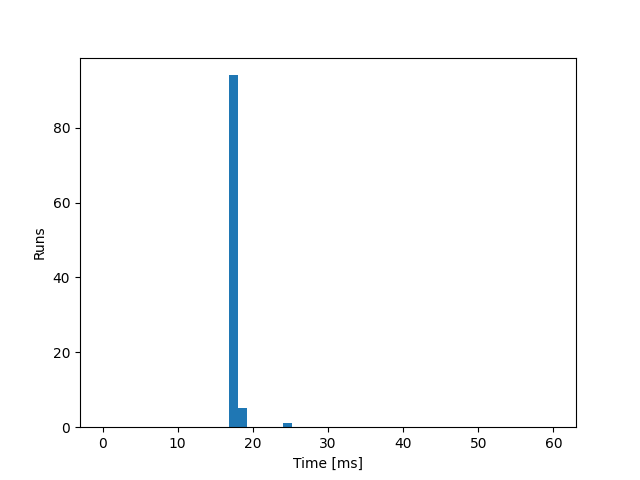
\includegraphics[width=\textwidth]{tests/sorting.wasmtime.png}
    \caption{Wasmtime}
  \end{subfigure}
  \begin{subfigure}[b]{0.32\textwidth}
    \centering
    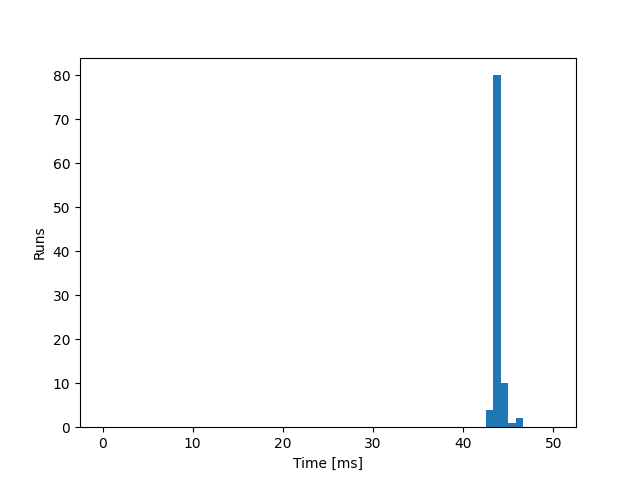
\includegraphics[width=\textwidth]{tests/sorting.wasm-landlock.png}
    \caption{WASM + Landlock}
  \end{subfigure}
  \begin{subfigure}[b]{0.32\textwidth}
    \centering
    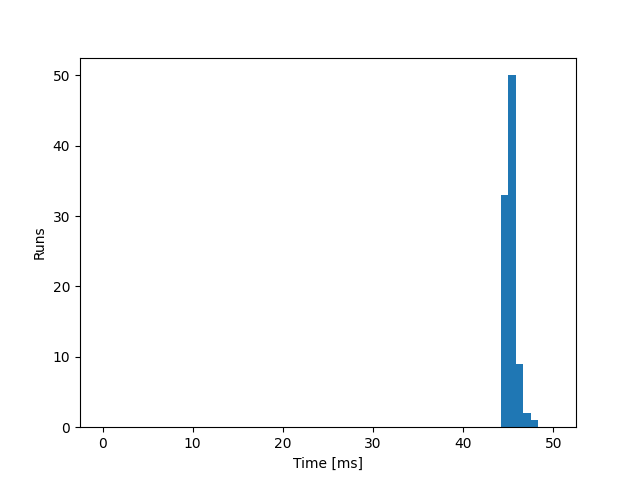
\includegraphics[width=\textwidth]{tests/sorting.wasm-bpf.png}
    \caption{WASM + eBPF}
  \end{subfigure}
  \caption{Distribution of execution times when sorting 10000 numbers (WASM).}
  \label{fig:distribution-sorting-wasm}
\end{figure}

\subsection{File system access}

\begin{figure}[h]
  \centering
  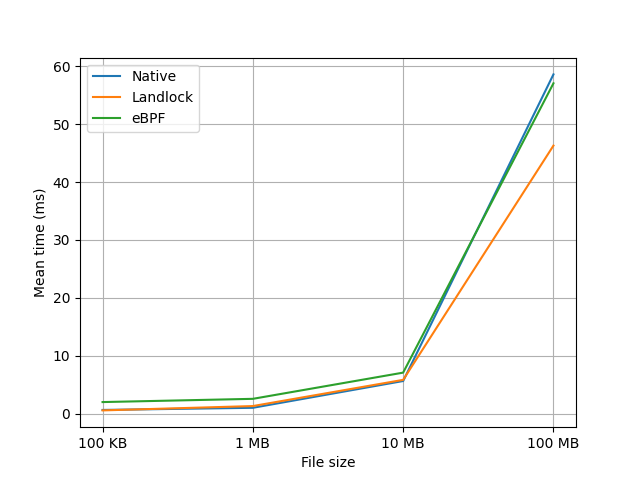
\includegraphics[width=0.8\linewidth]{tests/reading-file-native-graph.png}
  \caption{A comparison of native average speeds when reading a file.}
  \label{fig:avg-comparison-native-speed}
\end{figure}

\begin{figure}[ht!]
  \centering
  \begin{subfigure}[b]{0.32\textwidth}
    \centering
    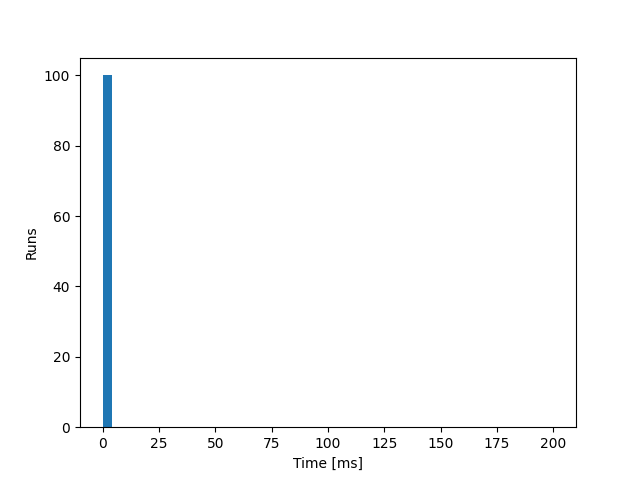
\includegraphics[width=\textwidth]{tests/reading-file-100k.native.png}
    \caption{Native (100 KB)}
  \end{subfigure}
  \begin{subfigure}[b]{0.32\textwidth}
    \centering
    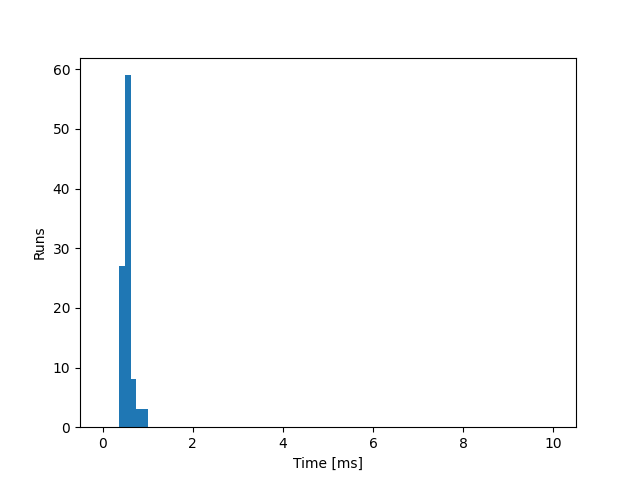
\includegraphics[width=\textwidth]{tests/reading-file-100k.native-landlock.png}
    \caption{Landlock (100 KB)}
  \end{subfigure}
  \begin{subfigure}[b]{0.32\textwidth}
    \centering
    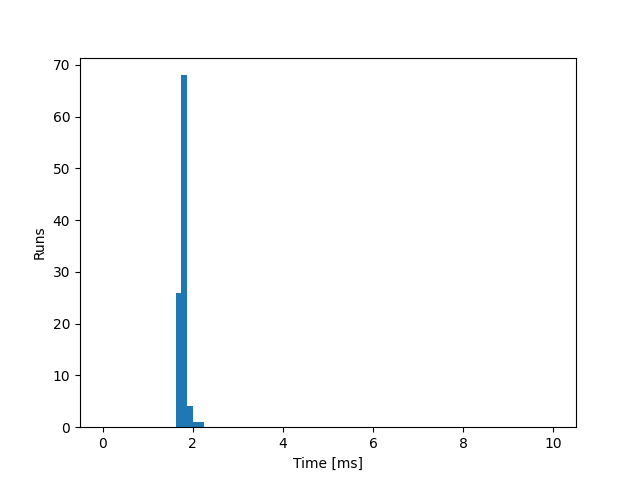
\includegraphics[width=\textwidth]{tests/reading-file-100k.native-bpf.png}
    \caption{eBPF (100 KB)}
  \end{subfigure}

  \begin{subfigure}[b]{0.32\textwidth}
    \centering
    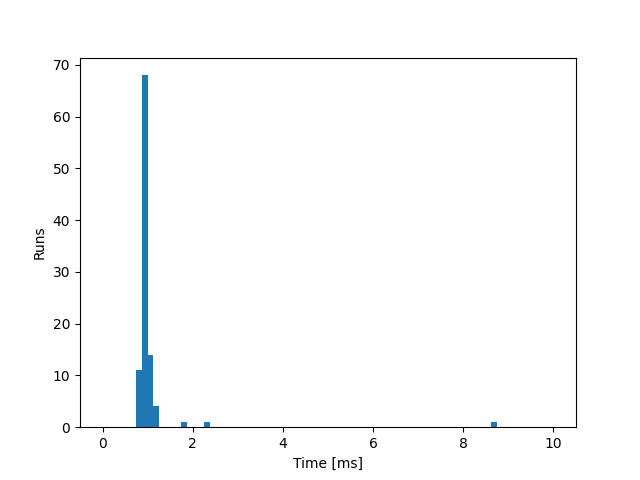
\includegraphics[width=\textwidth]{tests/reading-file-1M.native.png}
    \caption{Native (1 MB)}
  \end{subfigure}
  \begin{subfigure}[b]{0.32\textwidth}
    \centering
    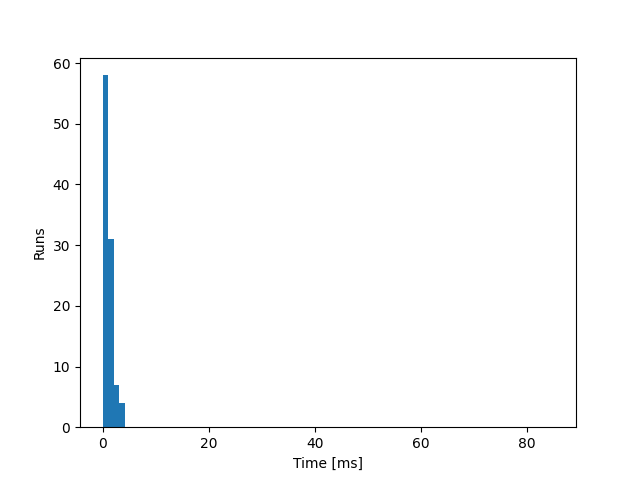
\includegraphics[width=\textwidth]{tests/reading-file-1M.native-landlock.png}
    \caption{Landlock (1 MB)}
  \end{subfigure}
  \begin{subfigure}[b]{0.32\textwidth}
    \centering
    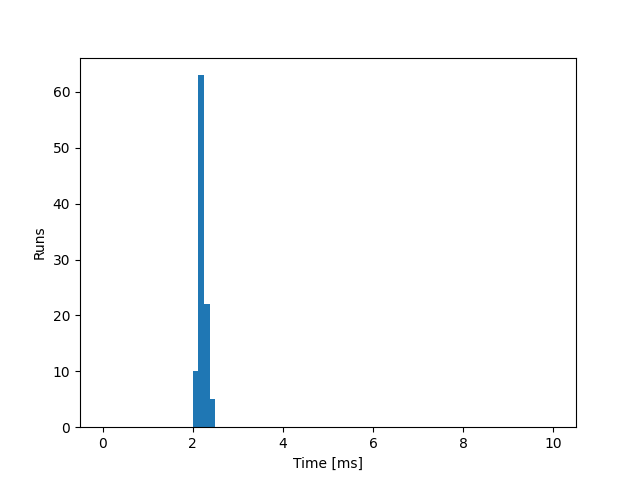
\includegraphics[width=\textwidth]{tests/reading-file-1M.native-bpf.png}
    \caption{eBPF (1 MB)}
  \end{subfigure}

  \begin{subfigure}[b]{0.32\textwidth}
    \centering
    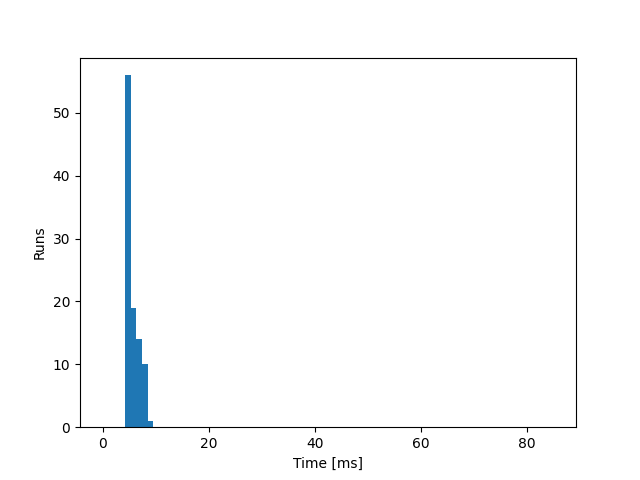
\includegraphics[width=\textwidth]{tests/reading-file-10M.native.png}
    \caption{Native (10 MB)}
  \end{subfigure}
  \begin{subfigure}[b]{0.32\textwidth}
    \centering
    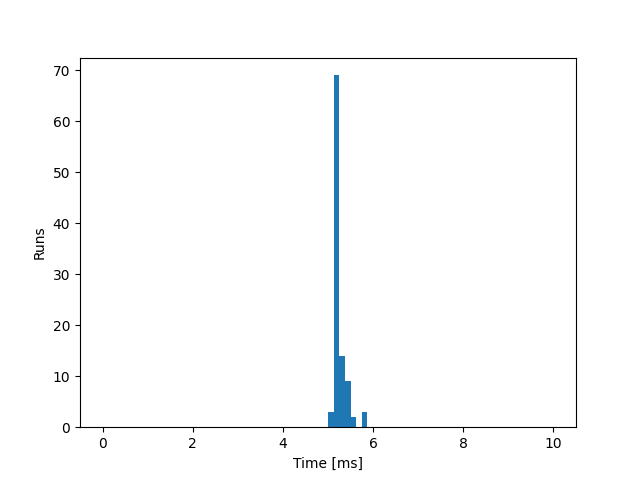
\includegraphics[width=\textwidth]{tests/reading-file-10M.native-landlock.png}
    \caption{Landlock (10 MB)}
  \end{subfigure}
  \begin{subfigure}[b]{0.32\textwidth}
    \centering
    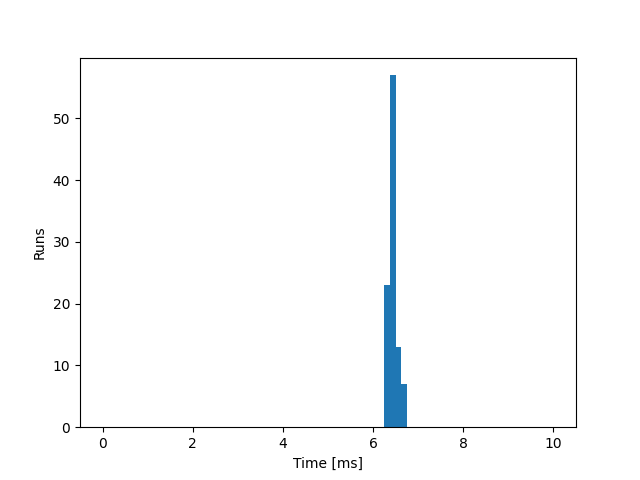
\includegraphics[width=\textwidth]{tests/reading-file-10M.native-bpf.png}
    \caption{eBPF (10 MB)}
  \end{subfigure}

  \begin{subfigure}[b]{0.32\textwidth}
    \centering
    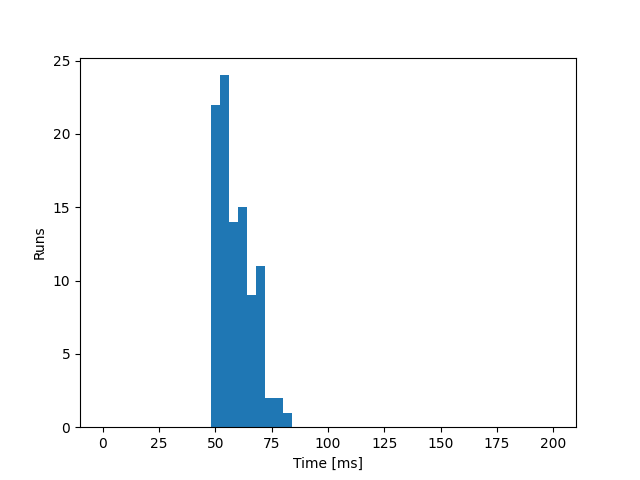
\includegraphics[width=\textwidth]{tests/reading-file-100M.native.png}
    \caption{Native (100 MB)}
  \end{subfigure}
  \begin{subfigure}[b]{0.32\textwidth}
    \centering
    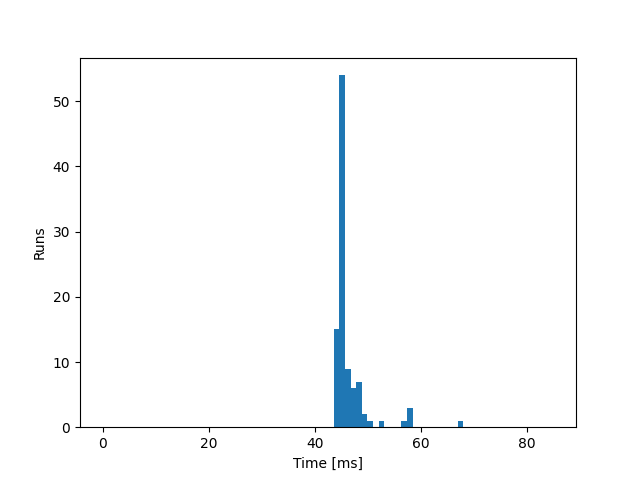
\includegraphics[width=\textwidth]{tests/reading-file-100M.native-landlock.png}
    \caption{Landlock (100 MB)}
  \end{subfigure}
  \begin{subfigure}[b]{0.32\textwidth}
    \centering
    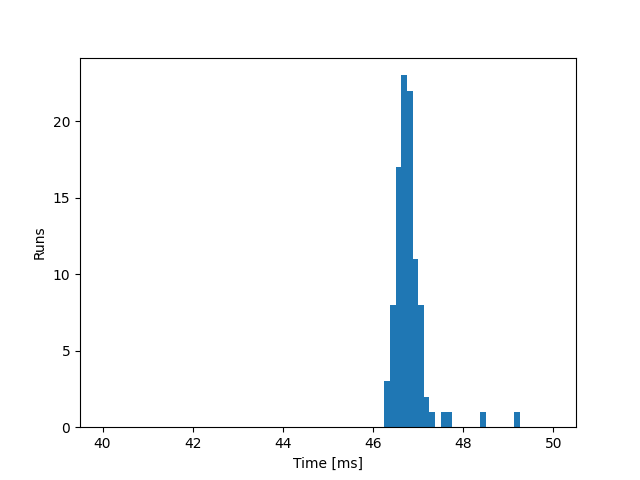
\includegraphics[width=\textwidth]{tests/reading-file-100M.native-bpf.png}
    \caption{eBPF (100 MB)}
  \end{subfigure}

  \caption{Distribution of a native binary execution times when reading a file.}
  \label{fig:distribution-reading-native}
\end{figure}


% The first thing of note, immediately shown by the data in Table \ref{table:lsm-impact-wasm},
% is that on average every single execution of a WASM binary, either restricted or not,
% is slower than running directly a native binary. This is also shown in the three distribution
% graphs visible in Figure \ref{fig:distribution-sorting-wasm}, especially when compared with
% the ones in Figure \ref{fig:distribution-sorting-native}.

% Hence, a WASM binary performance is reasonably comparable to a native binary,
% although there is a constant overhead of at least 20 ms in all the test runs.

% There is another interesting result that presents itself when analysing the integration of Landlock
% and the embedding of WebAssembly modules in Rust (through \textit{Wasmtime}) -
% a constant overhead with respect to using \textit{Wasmtime} directly or through eBPF.
% This can be seen in Table \ref{table:lsm-impact-wasm}, but is more visible in Figure \ref{fig:avg-comparison-wasm-speed},
% showing how the average execution time varies with respect to read file size -
% the \textit{Landlock} curve has roughly the same shape as the other two, but appears translated
% of a constant factor of around 30 ms.

% Since in Section \ref{sec:landlock-vs-ebpf-native} it was shown that no restriction method had a considerable overhead
% against a native binary, and because in this case the WASM module is interpreted by a native binary
% restricted with Landlock, it stands to reason that this overhead should be due to the usage
% of the library provided by \textit{Wasmtime} for integrating WASM in Rust.

% In all cases, however, execution times are not higher than 200 ms - although being a noticeable
% delay, this is small enough to not be of any discomfort to a human user.

\begin{figure}[ht!]
  \centering
  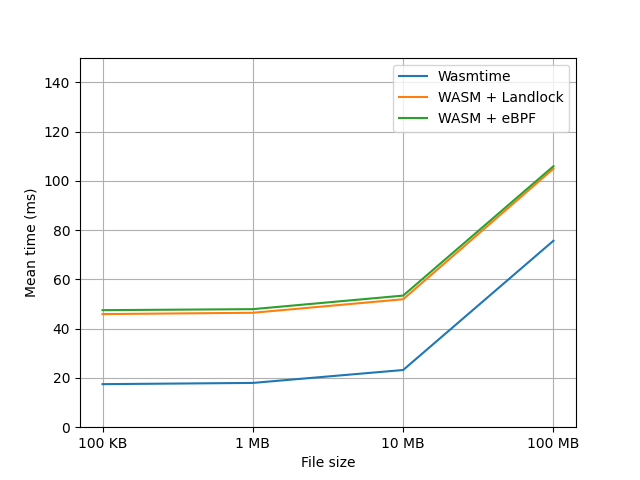
\includegraphics[width=0.8\linewidth]{tests/reading-file-wasm-graph.png}
  \caption{A comparison of WASM average speeds when reading a file.}
  \label{fig:avg-comparison-wasm-speed}
\end{figure}

\begin{figure}[ht!]
  \centering
  \begin{subfigure}[b]{0.32\textwidth}
    \centering
    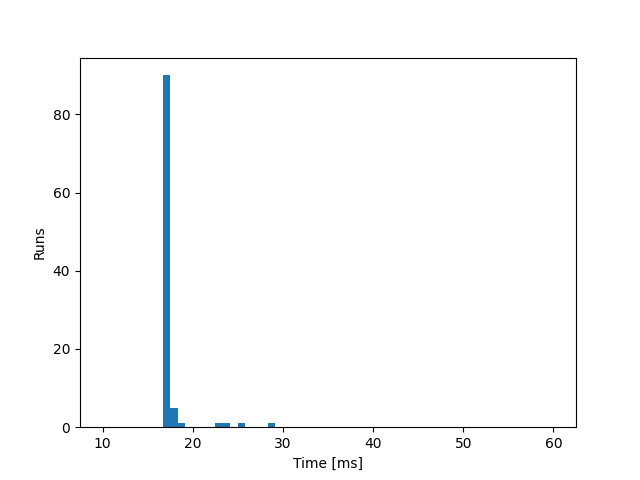
\includegraphics[width=\textwidth]{tests/reading-file-100k.wasmtime.png}
    \caption{Wasmtime (100 KB)}
  \end{subfigure}
  \begin{subfigure}[b]{0.32\textwidth}
    \centering
    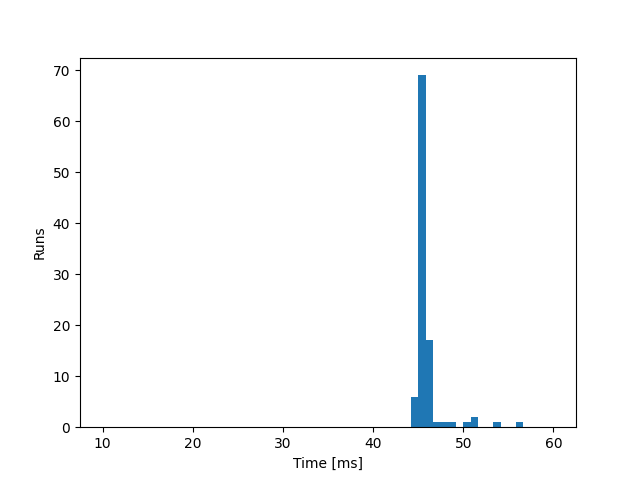
\includegraphics[width=\textwidth]{tests/reading-file-100k.wasm-landlock.png}
    \caption{Landlock (100 KB)}
  \end{subfigure}
  \begin{subfigure}[b]{0.32\textwidth}
    \centering
    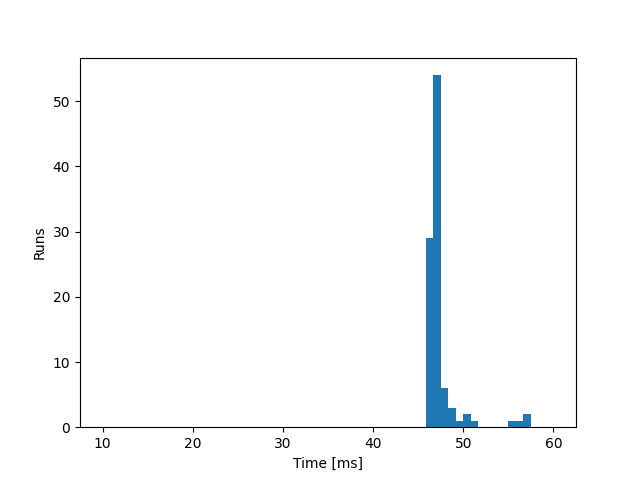
\includegraphics[width=\textwidth]{tests/reading-file-100k.wasm-bpf.png}
    \caption{eBPF (100 KB)}
  \end{subfigure}

  \begin{subfigure}[b]{0.32\textwidth}
    \centering
    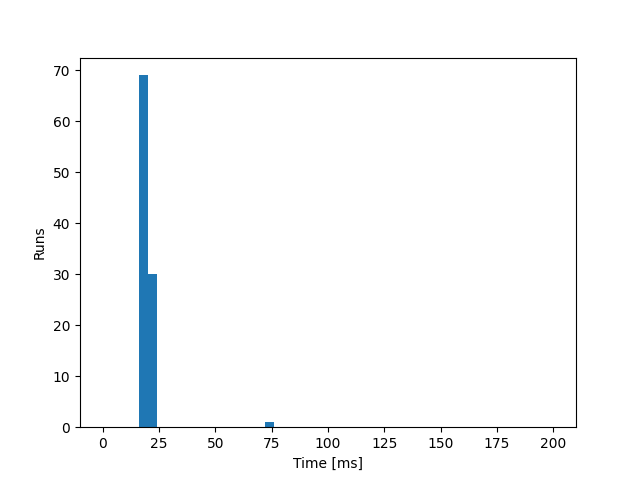
\includegraphics[width=\textwidth]{tests/reading-file-1M.wasmtime.png}
    \caption{Wasmtime (1 MB)}
  \end{subfigure}
  \begin{subfigure}[b]{0.32\textwidth}
    \centering
    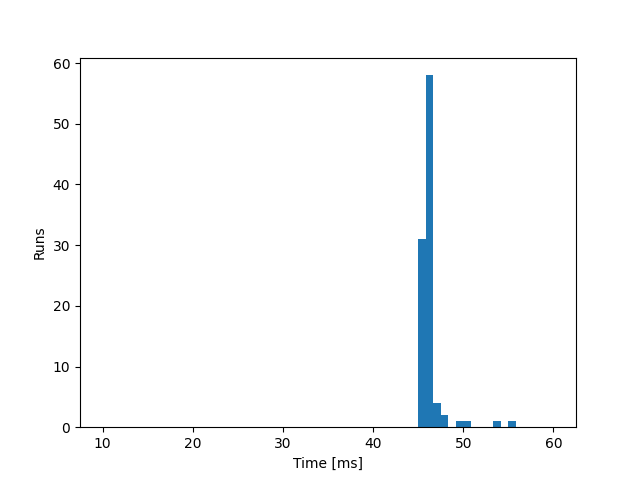
\includegraphics[width=\textwidth]{tests/reading-file-1M.wasm-landlock.png}
    \caption{Landlock (1 MB)}
  \end{subfigure}
  \begin{subfigure}[b]{0.32\textwidth}
    \centering
    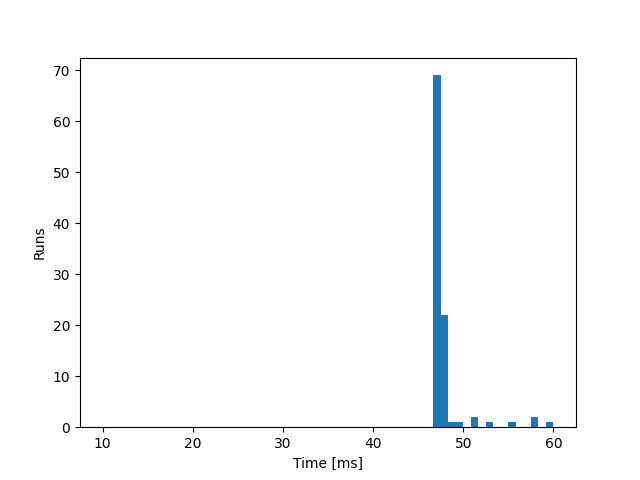
\includegraphics[width=\textwidth]{tests/reading-file-1M.wasm-bpf.png}
    \caption{eBPF (1 MB)}
  \end{subfigure}

  \begin{subfigure}[b]{0.32\textwidth}
    \centering
    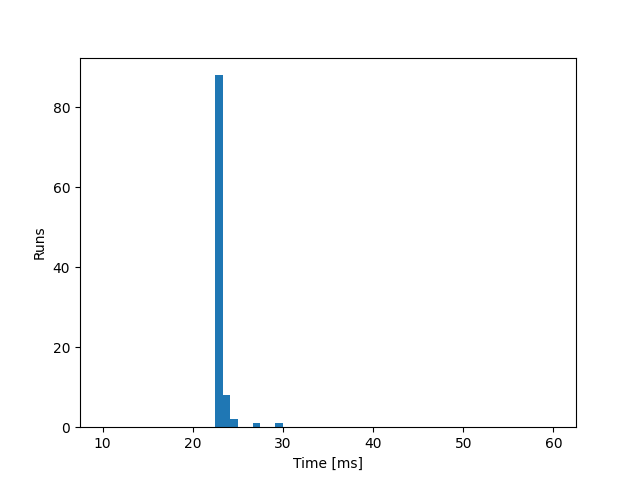
\includegraphics[width=\textwidth]{tests/reading-file-10M.wasmtime.png}
    \caption{Wasmtime (10 MB)}
  \end{subfigure}
  \begin{subfigure}[b]{0.32\textwidth}
    \centering
    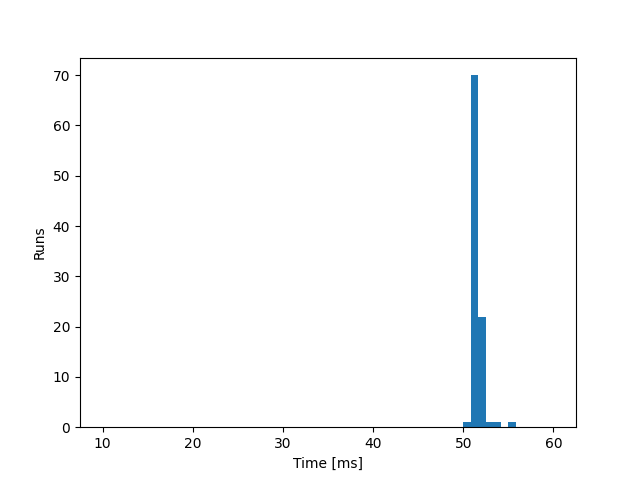
\includegraphics[width=\textwidth]{tests/reading-file-10M.wasm-landlock.png}
    \caption{Landlock (10 MB)}
  \end{subfigure}
  \begin{subfigure}[b]{0.32\textwidth}
    \centering
    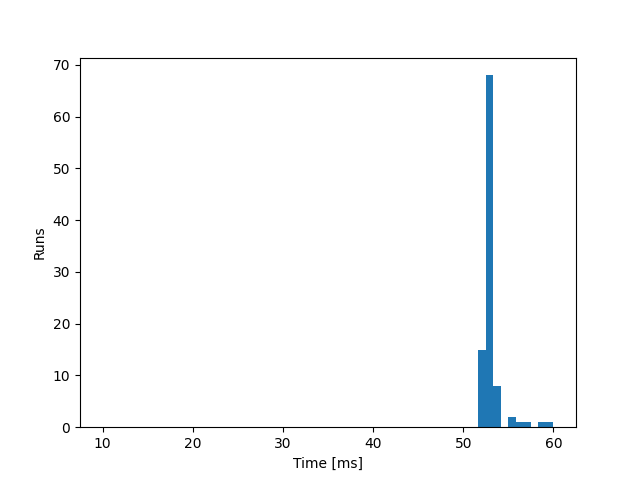
\includegraphics[width=\textwidth]{tests/reading-file-10M.wasm-bpf.png}
    \caption{eBPF (10 MB)}
  \end{subfigure}

  \begin{subfigure}[b]{0.32\textwidth}
    \centering
    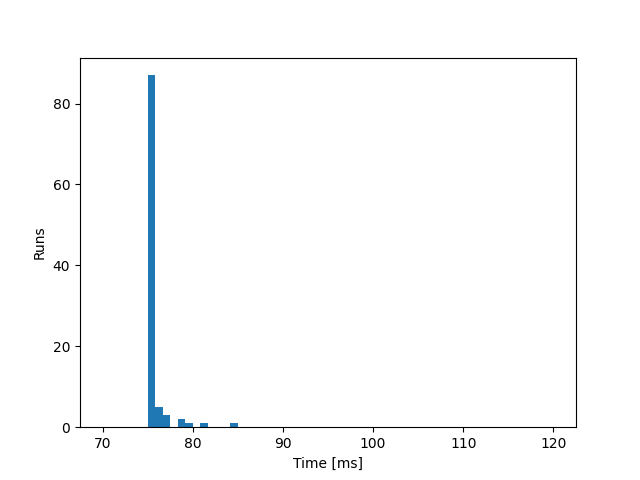
\includegraphics[width=\textwidth]{tests/reading-file-100M.wasmtime.png}
    \caption{Wasmtime (100 MB)}
  \end{subfigure}
  \begin{subfigure}[b]{0.32\textwidth}
    \centering
    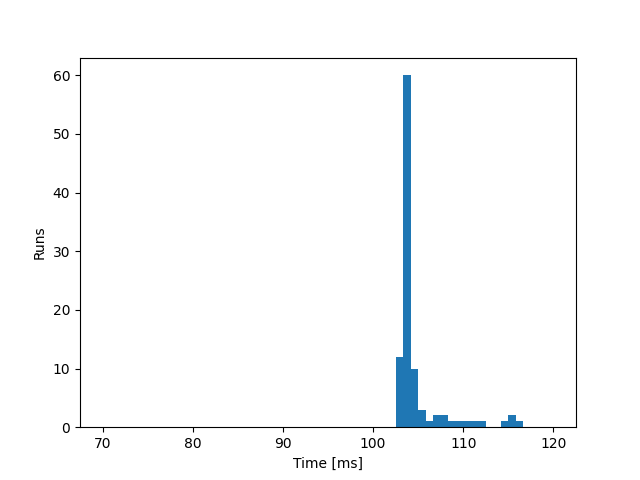
\includegraphics[width=\textwidth]{tests/reading-file-100M.wasm-landlock.png}
    \caption{Landlock (100 MB)}
  \end{subfigure}
  \begin{subfigure}[b]{0.32\textwidth}
    \centering
    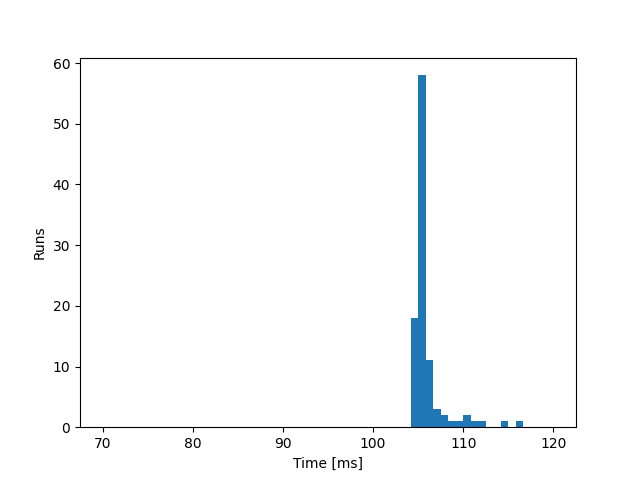
\includegraphics[width=\textwidth]{tests/reading-file-100M.wasm-bpf.png}
    \caption{eBPF (100 MB)}
  \end{subfigure}

  \caption{Distribution of a WASM binary execution times when reading a file.}
  \label{fig:distribution-reading-wasm}
\end{figure}

\section{Internal analysis of the developed project}

In order to test the performance of the integration between Landlock and WebAssembly,
embedded in Rust through WebAssembly, through the use of the standard library \texttt{std::time::Instant}
various timestamps were taken and then combined in order to measure the execution time of various program parts.
A total of 100 runs were used in order to measure the average execution times.

Two different WebAssembly programs were tested - a trivial one
(Listing \ref{lst:project-perf-program-simple}) and a more complex one, with
file system access and specific restrictions enabled (Listing \ref{lst:project-perf-program-complex}).
Both these programs were compiled with \texttt{rustc} with a \texttt{wasm32-wasi} target and full
optimisations enabled.

\vspace*{0.5cm}

\begin{code}[language=Rust, caption=The tested trivial program, label=lst:project-perf-program-simple]
  fn main() {
    println!("Hello World");
  }
\end{code}

\clearpage
\begin{code}[language=Rust, caption=The more complex tested program, label=lst:project-perf-program-complex]
use std::fs::{read_to_string, write};

fn main() {
  read_to_string("file1.txt")
    .expect("Could not read file1");
  write("file1.txt", "New content 1")
    .expect("Could not write file1");
  read_to_string("subdir/file2.txt")
    .expect("Could not read file2");
  write("subdir/file2.txt", "New content 2")
    .expect("Could not write file2");
}  
\end{code}

\subsection{Execution times}

The different program parts considered in these measures are the following:
\begin{itemize}
  \item argument parsing;
  \item WASM module instantiation;
  \item the preopening of all directories by Wasmtime;
  \item applying all the Landlock rules;
  \item and finally, compiling and running the WASM module.
\end{itemize}

\begin{table}
  \centering
  \csvreader[
    tabular={|l|r|r|r|r|},
    table head = \hline
      \textit{Program part} & $\mu_\mathrm{Instant}$ & $\sigma_\mathrm{Instant}$ & $\mu_\mathrm{Cumulative}$ & $\sigma_\mathrm{Cumulative}$   \\ \hline\hline,
    late after line = \\ \hline,
    head to column names,
  ]{test-data/project-stats-simple.csv}{}
  {\type & \mean & \stddev & \meanc & \stddevc}
  \caption{Execution times in $\mu s$ when running the simple program (Listing \ref{lst:project-perf-program-simple}).}
  \label{table:execution-times-simple}
\end{table}

\begin{table}
  \centering
  \csvreader[
    tabular={|l|r|r|r|r|},
    table head = \hline
      \textit{Program part} & $\mu_\mathrm{Instant}$ & $\sigma_\mathrm{Instant}$ & $\mu_\mathrm{Cumulative}$ & $\sigma_\mathrm{Cumulative}$   \\ \hline\hline,
    late after line = \\ \hline,
    head to column names,
  ]{test-data/project-stats-medium.csv}{}
  {\type & \mean & \stddev & \meanc & \stddevc}
  \caption{Execution times in $\mu s$ when running the complex program (Listing \ref{lst:project-perf-program-complex}).}
  \label{table:execution-times-complex}
\end{table}

In Table \ref{table:execution-times-simple} and Table \ref{table:execution-times-complex} are visible
both the average time spent by a program section ($\mu_\mathrm{Instant}$) and the cumulative time
up until that same section ($\mu_\mathrm{Cumulative}$), all measured in microseconds.
For example, if the part ``Landlock enforcement'' is such that $\mu_\mathrm{Instant} = 20$ and $\mu_\mathrm{Cumulative} = 100$,
this means that on average it takes 20 $\mu s$ to apply Landlock to the running process, and on average this part
is fully completed after 100 $\mu s$ from the beginning of the program.

As is shown in both Table \ref{table:execution-times-simple} and Table \ref{table:execution-times-complex},
the performance impact of using Landlock to restrict the binary is negligible.
The biggest bottleneck is given by running the WebAssembly binary - more specifically, instantiating
the required engine and linker, and then interpreting and running the WASM module (as specified in Section \ref{sec:landlock-wasm-module}).

Moreover, this data confirms the hypothesis brought forward in Section \ref{sec:landlock-vs-ebpf-wasm} - that
the constant overhead presented by running WASM in combination with Landlock must be due to the usage of
the WASI embedding library provided by \textit{Wasmtime}, and not a byproduct of restricting the process with Landlock.

Finally, Figure \ref{fig:perf-execution-times-comparison} shows how each program section
occupies the overall time spent running by the program. The various labels are as follows
- \texttt{A} is for ``Argument parsing'', \texttt{B} is for ``Module initialisation'',
\texttt{C} is for ``Preopen'', \texttt{D} is for ``Landlock enforcement'' and
\texttt{E} is for ``Running WASM binary''.

\begin{figure}[ht!]
  \centering
  
  \begin{subfigure}[b]{0.46\textwidth}
    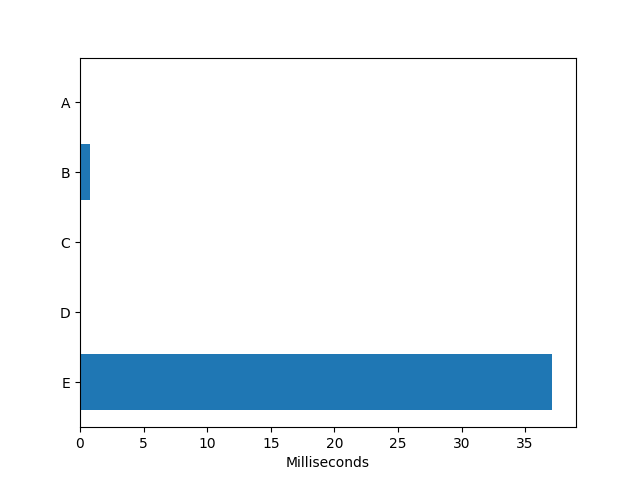
\includegraphics[width=\textwidth]{project-performance/graph_simple.png}
    \caption{Simple program}
  \end{subfigure}
  \begin{subfigure}[b]{0.46\textwidth}
    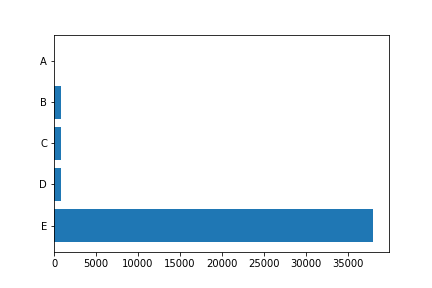
\includegraphics[width=\textwidth]{project-performance/graph_simple_c.png}
    \caption{Simple program (cumulative)}
  \end{subfigure}

  \begin{subfigure}[b]{0.46\textwidth}
    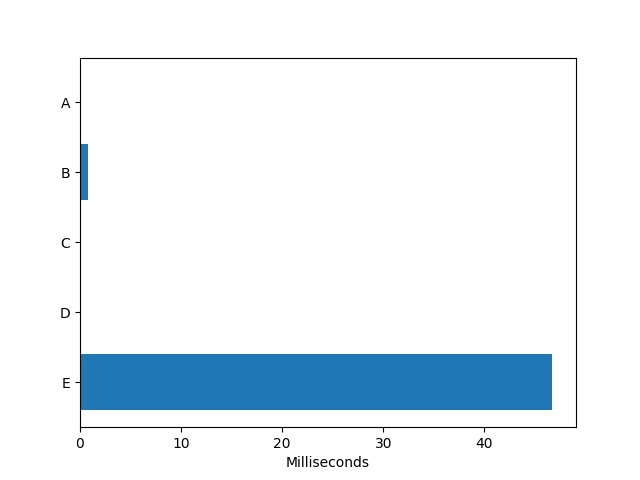
\includegraphics[width=\textwidth]{project-performance/graph_medium.png}
    \caption{Complex program}
  \end{subfigure}
  \begin{subfigure}[b]{0.46\textwidth}
    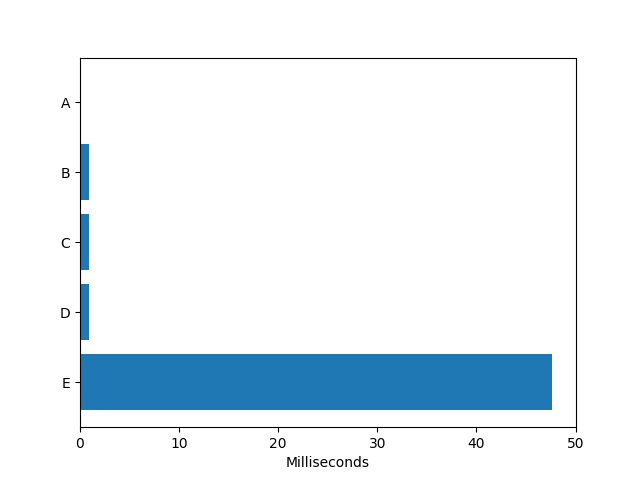
\includegraphics[width=\textwidth]{project-performance/graph_medium_c.png}
    \caption{Complex program (cumulative)}
  \end{subfigure}

  \caption{A graphic comparison of all the execution times, in $\mu s$.}
  \label{fig:perf-execution-times-comparison}
\end{figure}

\section{Conclusions and observations}